\chapter{Arquitetura para compartilhamento de informações do ativo}
\label{cha:arquitetura}

A elaboração de uma arquitetura comum para o compartilhamento de informações de um ativo é essencial para que haja consistência e interoperabilidade entre os membros da Cadeia de Suprimentos (CS) adotando este sistema.

Este capítulo tem o objetivo de apresentar detalhes da arquitetura proposta baseada em \textit{Web Services} (WS) nos modelos de uma arquitetura orientada a serviços (SOA) compatível com Componentes I4.0 para o compartilhamento de informações do ativo ao longo da CS. A fim de simplificação do texto, os \textit{Web Services} serão mencionados apenas como ``serviços''.

Neste capítulo é apresentado também o mapeamento dos componentes desta arquitetura dentro do eixo camadas do RAMI4.0.

\section{Componentes e operações dos serviços de AASs}
\label{sec:componentes-e-operacoes}

Os serviços no escopo desta arquitetura são representações das funcionalidades dos Componentes I4.0 e são fornecidos e consumidos entre \textit{Asset Administration Shells} (AAS), ou, de forma mais geral, entre os Componentes I4.0 (C4.0), que englobam o AAS.

A lógica de fornecimento e consumo de serviços proposta para a I4.0 segue os moldes de um \textit{Web Service} detalhado na \autoref{sub:web-services}, onde foram apresentados os componentes e operações (vide \autoref{fig:webservice-componentes}) adaptados ao AAS.

Esta arquitetura envolve três Componentes I4.0 (C4.0) ou atores básicos: O C4.0-Cliente, o C4.0-Servidor e o C4.0-Repositório; e três operações: publicação, busca e interação.

Os serviços disponibilizados remotamente pelo C4.0-Servidor escutam e respondem solicitações de clientes por meio de uma determinada rede e porta. Os C4.0-Clientes, por sua vez, consomem o serviço disponibilizado pelo C4.0-Servidor por meio de solicitações.

Nesta seção são apresentados detalhes sobre os Componentes I4.0 e as operações necessárias para o fornecimento de serviços no mundo conectado da I4.0.

\subsection{Componentes}

Os Componentes I4.0 (C4.0) da arquitetura e suas inter-relações são apresentados na \autoref{fig:aas-ws}.

\begin{figure}[htb]
	\centering
	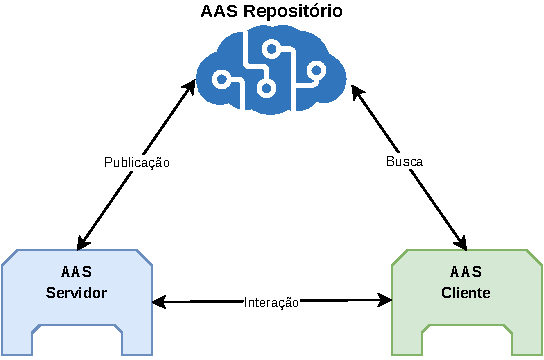
\includegraphics[width=0.7\textwidth]{aas-ws}
	\caption{Componentes e operações do WS.}
	\label{fig:aas-ws}
\end{figure}

De maneira sucinta, os C4.0 são descritos da seguinte forma: ``C4.0-Servidor'' é a parte que possui um serviço a oferecer para os demais C4.0s no mundo conectado, o ``C4.0-Cliente'' é a parte que necessita de um serviço e que age ativamente para receber este serviço e o ``C4.0-Repositório'' é a parte que armazena informações sobre descrições de diversos serviços, que são disponibilizados na forma de contratos.

A \autoref{tab:componentes-ws} lista os C4.0 da arquitetura e suas respectivas descrições detalhadas.

\begin{table}[htb]
	\centering
	\caption{Componentes da arquitetura proposta.}
	\label{tab:componentes-ws}
	\begin{tabular}{p{3cm}p{12cm}}
		\hline
		\textbf{Componente}
		 & \textbf{Descrição}                                                                                                                                                                                                                                                                                                                                                                                                                                                                                                                                                                               \\

		\hline
		C4.0-Servidor
		 & O C4.0-Servidor é fonte de informações. Este C4.0 extrai as informações sobre seu ativo para sua própria MDP para que assim possam ser disponibilizadas na rede. Cada submodelo do AAS representa um conjunto de informações e serviços semelhantes agrupados.                                                                                                                                                                                                                                                                                                                                   \\

		\hline
		C4.0-Cliente
		 & O C4.0-Cliente é a parte que irá consumir as informações disponibilizadas pelo C4.0-Servidor. O cliente representa cada uma das partes envolvidas na cadeia de suprimentos. Pode representar uma instituição, uma pessoa física ou até mesmo uma outra máquina/produto.                                                                                                                                                                                                                                                                                                                          \\

		\hline
		C4.0-Repositório
		 & O C4.0-Repositório é o elemento que recebe, armazena e disponibiliza informações de descrição sobre todos os serviços disponíveis no mundo conectado, as descrições de serviços são disponibilizados em forma de contratos. Este componente recebe operações de ``publicação'' por parte do C4.0-Servidor e operações de ``busca'' por parte do C4.0-Cliente. O C4.0-Repositório não atua como canal de comunicação entre C4.0-Cliente e C4.0-Servidor, mas apenas fornece informações necessárias para que ambos os C4.0 possam se comunicar diretamente por meio da operação de ``interação''. \\

		\hline
	\end{tabular}
\end{table}

Neste modelo, o contrato contendo a descrição dos serviços disponíveis nos submodelos de cada C4.0-Servidor é armazenado em um repositório comum, onde todos os C4.0 disponíveis no mundo conectado na I4.0 podem se tornar visíveis. O serviço é fornecido pelo próprio C4.0-Servidor que o tornou público, servindo o repositório apenas como um elemento para a descoberta de serviços.

É importante notar que no mundo da I4.0 todo ativo é englobado por um AAS e se torna um Componente I4.0. Como o repositório detém informações e funções que agregam valor ao negócio, este pode também ser considerado um ativo, que no caso é o \textit{software} que gerencia os relacionamentos das descrições dos serviços. O C4.0-Repositório então engloba este ativo para dar a capacidade de interação com outros C4.0 na Indústria 4.0.

Cada C4.0 pode atuar tanto como um fornecedor de serviços (servidor), quanto como um solicitante de serviços (cliente), ou como ambos. Sempre usando o repositório como meio para a publicação ou busca dos serviços.

\subsection{Operações}

As descrições das operações dos serviços são apresentadas na \autoref{tab:operacoes-ws}. As inter-relações entre C4.0s por meio das operações são mostradas na \autoref{fig:aas-ws}.

\begin{table}[htb]
	\centering
	\caption{Operações do WS para a interação entre C4.0s.}
	\label{tab:operacoes-ws}
	\begin{tabular}{p{3cm}p{12cm}}
		\hline
		\textbf{Operação}
		 & \textbf{Descrição}                                                                                                                                                                                                                                                                                                                                                                                                                                                \\

		\hline
		Publicação
		 & Ação tomada pelo C4.0-Servidor sempre que este queira anunciar um serviço para que possa ser descoberto por um C4.0-Cliente. Nesta operação, o C4.0-Servidor envia o contrato descrevendo os serviços ofertados e a descrição de cada um desses serviços. Esta lista é recebida e armazenada pelo C4.0-Repositório, que a disponibiliza para acesso público.                                                                                                      \\

		\hline
		Busca
		 & Ação tomada pelo C4.0-Cliente sempre que este precise consultar serviços de seu interesse. Nesta operação o C4.0-Cliente faz uma solicitação ao C4.0-Repositório com os parâmetros que definem o tipo e as restrições do serviço desejado. A operação de busca engloba também o fluxo contrário de informações, que é o envio da resposta da solicitação do C4.0-Repositório para o C4.0 Cliente.                                                                 \\

		\hline
		Interação
		 & Ação tomada pelo C4.0-Cliente sempre que este deseja invocar um serviço. O C4.0-Cliente estabelece uma conexão direta com o C4.0-Servidor e consome o determinado serviço solicitado. A operação de interação normalmente é feita após o recebimento da lista de contratos por parte do C4.0-Repositório, porém a interação pode ser feita diretamente caso o C4.0-Cliente já possua informações necessárias para o estabelecimento da conexão em \textit{cache}. \\

		\hline
	\end{tabular}
\end{table}

Para cada uma das operações deve ser definido o contrato, documento o qual descreve as funcionalidades do \textit{Web Service} e estabelece os padrões de comunicação suportados pelo C4.0-Servidor como, por exemplo, o padrão HTTP REST, HTTP SOAP, gRPC, etc; e especifica como acessar e quais são as operações ou métodos que estão disponíveis no serviço.

Quando o C4.0 atua como Servidor, este publica seu contrato no repositório por meio de uma API (\textit{Application Programming Interface}). Quando atua como Cliente, o C4.0 busca no repositório um serviço desejado e recebe uma lista de opções de serviços com suas respectivas descrições (contidas no contrato). Assim, o serviço mais adequado pode ser selecionado.

Uma vez definido o serviço a ser consumido, o C4.0-Cliente estabelecerá a conexão direta com o C4.0-Servidor por meio de algum dos padrões suportados, utilizando os detalhes contidos no contrato para localizar, contactar e invocar o serviço.

A \autoref{fig:pfs-ws} apresenta um diagrama PFS (\textit{Production Flow Schema}) (vide \autoref{sec:modelagem-de-sistemas}), com o fluxo de ocorrência das operações básicas no WS para a interação entre C4.0s.

\begin{figure}[htb]
	\centering
	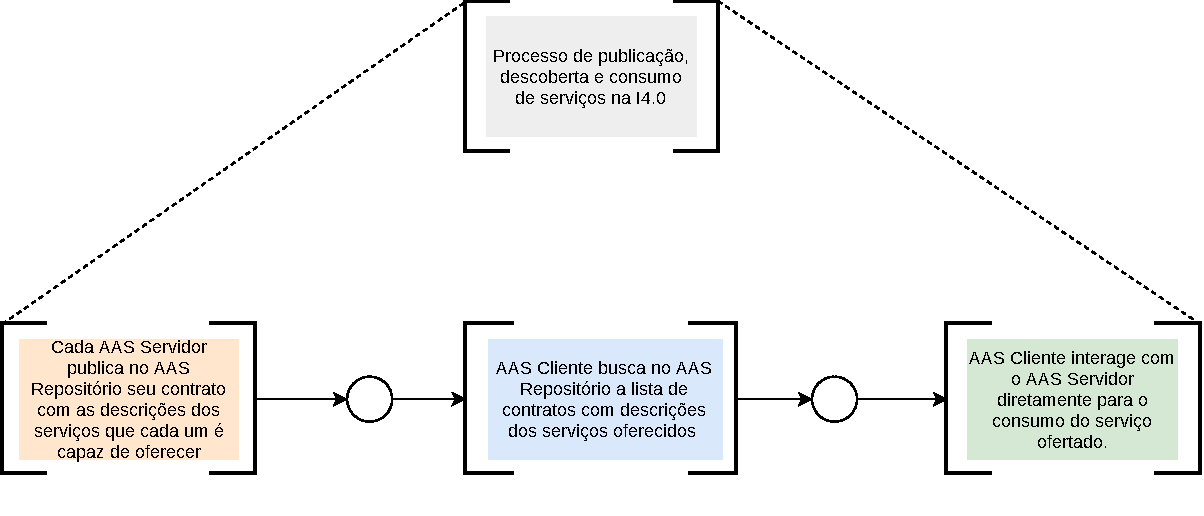
\includegraphics[width=1\textwidth]{pfs-ws}
	\caption{Diagrama PFS das operações do WS.}
	\label{fig:pfs-ws}
\end{figure}

Os serviços fornecidos por um C4.0 são diversos. Entretanto, neste trabalho serão tratados com ênfase aqueles serviços que têm como objetivo o compartilhamento de informações sobre o ativo que possam agregar valor ao produto ao longo de sua cadeia de suprimentos. Ou seja, os serviços que extraem informações da MDP do C4.0 e as fornecem, mediante autenticação, às partes solicitantes ao longo da cadeia de suprimentos.

\section{Fluxo de fornecimento de serviços}
\label{sec:fluxo-de-fornecimento-de-servicos}

As etapas para o fornecimento de serviços na I4.0 segue um fluxo padrão. Os submodelos agregam informações semelhantes que podem ser lidas ou escritas (via MDP) e disponibilizada por meio de \textit{Web Services} a qualquer uma das partes ao longo da CS mediante autenticação.

Um fluxo de leitura/escrita de dados pode ser exemplificado com uma CS simples contendo três membros: um fabricante, um distribuidor e um consumidor; cada membro da CS é um C4.0-Cliente diferente. O fabricante cria o produto, que será o C4.0-Servidor, e define a estrutura do AAS com os submodelos necessários (vide \autoref{sec:submodelos-produto}). A título de exemplo, três submodelos são definidos: submodelo ``Pedido'', submodelo ``Operação'' e submodelo ``Documentação''. Ao longo do ciclo de vida do produto, os membros da CS (fabricante, distribuidor e consumidor) podem interagir com esses submodelos, fazendo sua leitura para o caso dos submodelos de pedido e operação, e podendo fazer a leitura e/ou escrita para o caso do submodelo de documentação.

A \autoref{fig:webservice-multielo} demonstra este cenário mencionado com o fluxo de operações básicas do WS em funcionamento. Neste exemplo, o (\textbf{a}) C4.0-Servidor de um produto mantém contato com o (\textbf{b}) C4.0-Cliente da empresa do fabricante, com o (\textbf{c}) C4.0-Cliente da empresa do distribuidor, e com o (\textbf{d}) C4.0-Cliente do consumidor final, fornecendo o serviço de consulta de informações de diferentes submodelos para cada um dos solicitantes.

\begin{figure}[htb]
	\centering
	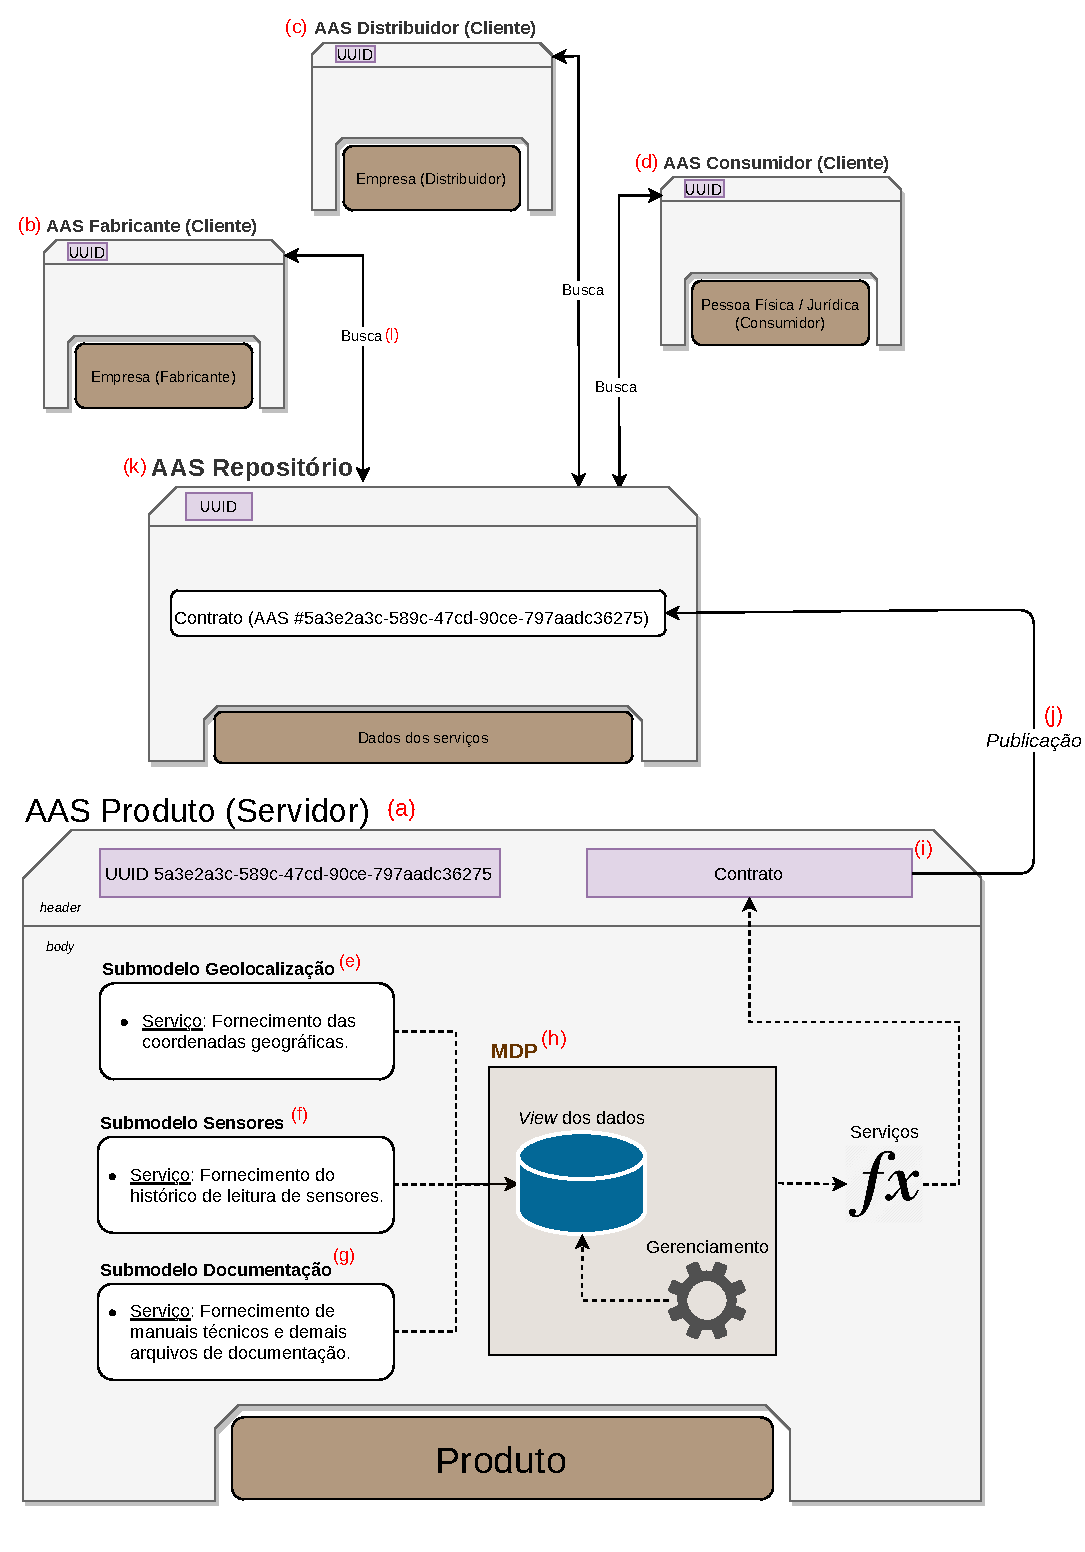
\includegraphics[width=0.75\textwidth]{webservice-multielo}
	\caption{Exemplificação das operações de publicação e busca com múltiplos clientes.}
	\label{fig:webservice-multielo}
\end{figure}

Na \autoref{fig:webservice-multielo} são mostrados os três submodelos do C4.0-Produto: (\textbf{e}) Submodelo ``Pedido'', (\textbf{f}) submodelo ``Operação'' e (\textbf{g}) submodelo ``Documentação''. A (\textbf{h}) MDP realiza o gerenciamento dos dados de todos os submodelos e os disponibiliza para acesso pelos serviços, as descrições dos serviços são armazenados em forma de um (\textbf{i}) contrato. Este contrato é (\textbf{j}) publicado no repositório.

O (\textbf{k}) C4.0-Repositório recebe o contrato do C4.0-Produto e o disponibiliza para consulta. O C4.0-Repositório poderá receber também contratos de diversos outros C4.0s do mundo conectado da I4.0.

Os C4.0-Clientes fazem a (\textbf{l}) busca no C4.0-Repositório. A requisição da busca é feita com parâmetros a fim de se restringir qual tipo de serviço aquele cliente pretende consumir, podendo-se restringir a busca, inclusive, ao serviço de um C4.0 específico, identificando-o por meio de seu UUID.

Cada C4.0-Cliente (Fabricante, Distribuidor ou Consumidor), portanto, realiza a consulta ao C4.0-Repositório com os parâmetros de interesse e recebe a resposta de contratos contendo descrições detalhadas sobre os serviços disponíveis e informações para localizar, contactar e invocar estes serviços.

Após o recebimento da resposta da busca pelo C4.0-Repositório, é feita a decisão interna em cada C4.0-Cliente sobre qual serviço selecionar. Uma vez definido, o C4.0-Cliente estabelece uma (\textbf{m}) interação com o C4.0-Servidor (produto), isto é, uma comunicação direta para o consumo do serviço selecionado.

Este é um exemplo de consulta única. Em aplicações reais, o cliente normalmente invocaria o serviço de diversos C4.0-Servidores ao mesmo tempo, como, por exemplo, um fabricante solicitando informações de todas as máquinas de um modelo específico que foram vendidas a clientes espalhados pelo mundo para realizar análise de dados a fim de se fazer a identificação de potenciais falhas e promover uma manutenção preditiva. Tal cenário é demonstrado em forma de um segundo exemplo na \autoref{fig:webservice-multiproduto}.

\begin{figure}[htb]
	\centering
	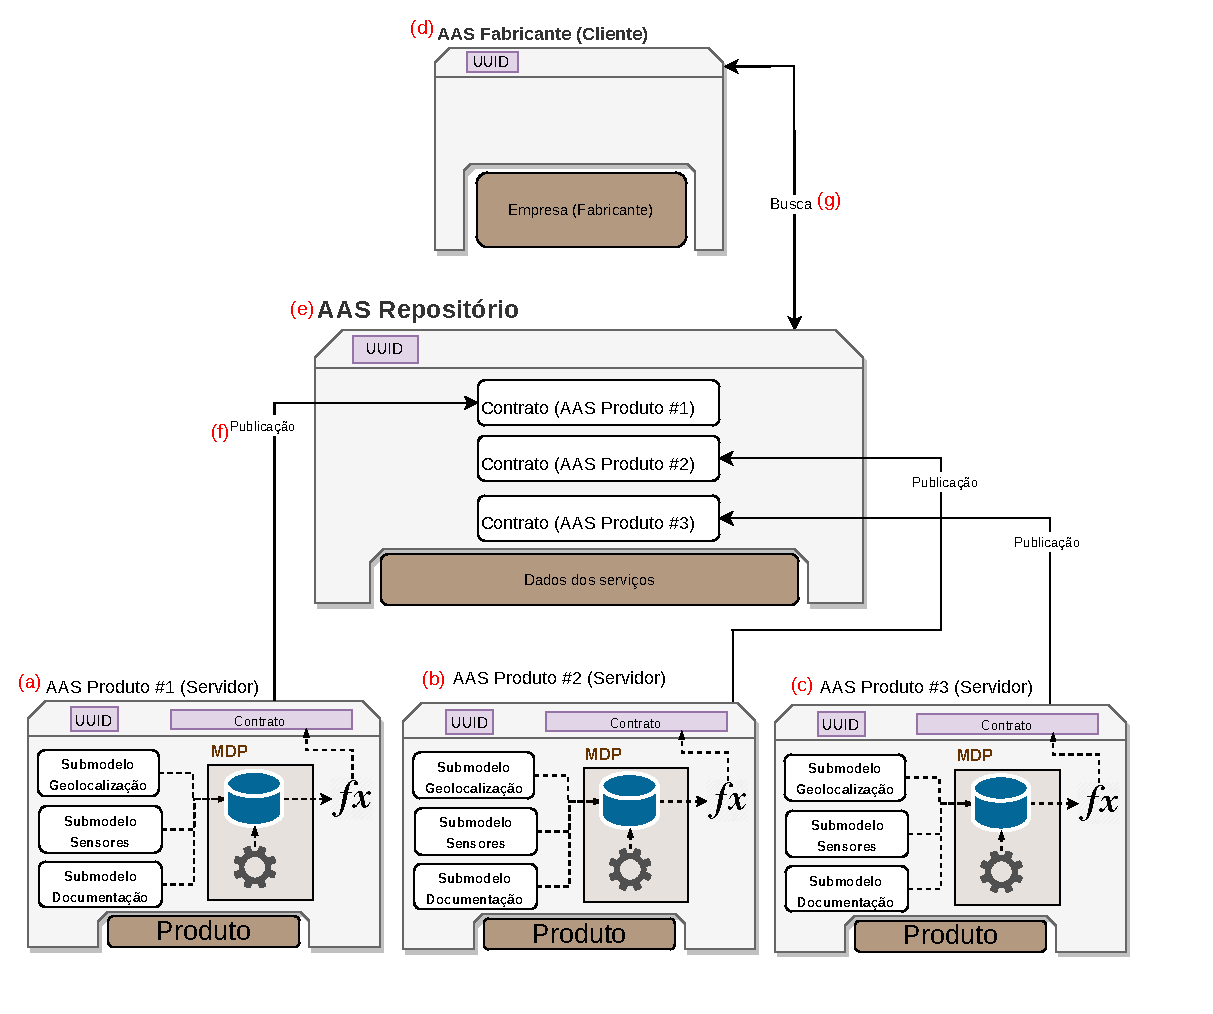
\includegraphics[width=1\textwidth]{webservice-multiproduto}
	\caption{Exemplificação das operações de publicação e busca com múltiplos produtos.}
	\label{fig:webservice-multiproduto}
\end{figure}

Neste cenário, há uma consulta por parte de um C4.0-Cliente a múltiplos produtos. Neste exemplo, cada C4.0-Produto (\textbf{a}, \textbf{b} e \textbf{c}) realiza uma operação de (\textbf{f}) publicação no (\textbf{e}) C4.0-Repositório.

O (\textbf{d}) C4.0-Cliente (fabricante) por sua vez faz uma (\textbf{g}) busca no C4.0-Repositório especificando os parâmetros que restrinjam a pesquisa a somente determinados modelos de produtos, e recebe como resposta todas as descrições dos serviços que correspondem aos critérios de busca.

A partir da resposta da busca no C4.0-Repositório, o C4.0-Cliente do fabricante pode (\textbf{h}) interagir diretamente com cada um dos C4.0-Servidores (produtos) para o consumo das informações necessárias.

\section{Mapeamento das operações no RAMI4.0}
\label{sec:mapeamento-das-operacoes}

Segundo \citeonline{iec2017rami}, o RAMI4.0 fornece uma visão estruturada dos principais elementos de um ativo usando um modelo de níveis composto por três eixos. Desta forma, inter-relações complexas podem ser divididas em seções menores e mais gerenciáveis, combinando os três eixos para representar cada aspecto relevante do estado do ativo em cada ponto de seu ciclo de vida.

Esta seção tem o objetivo de mapear as operações envolvidas nos fluxos de compartilhamento informações ao longo da cadeia de suprimentos para as camadas do RAMI4.0 de forma a representar as etapas relacionadas ao trânsito de informações em um modelo unificado.

O mapeamento para o RAMI4.0, que é uma arquitetura de referência para a I4.0, contribui para facilitar a execução de implementações de conceitos de I4.0 uma vez que estabelece um padrão de arquitetura que deve ser adotado por todos, garantindo a interoperabilidades entre os sistemas.

Nesta seção os termos C4.0-Cliente, C4.0-Servidor e C4.0-Repositório são utilizados para denotar os componentes completos, ou seja a junção do AAS com sua parte real (o ativo).

\subsection{Funcionalidades das camadas do RAMI4.0}

Na \autoref{sub:rami4} foram apresentados os detalhes do RAMI4.0 e o detalhamento de cada nível do eixo Camadas com suas funções genéricas. Nesta subseção são mostradas as funções específicas da arquitetura proposta para cada camada o sob o contexto do compartilhamento de informações pela CS.

Na camada \textbf{Ativo} estão os produtos (servidor de informações) e os clientes diversos (empresas, pessoas, consumidores das informações).

Para o compartilhamento de informações do produto no mundo I4.0, os dados a serem extraídos do ativo são estrategicamente selecionados com o objetivo de reunir somente os que agreguem valor ao próprio ativo. Assim, estes dados selecionados são extraídos do ativo e repassados às camadas superiores para que possam ser armazenados e compartilhados por meio de serviços.

A camada \textbf{Integração} está presente em todos os componentes (Servidor, Cliente e Repositório). Porém tanto o C4.0-Cliente quanto o C4.0-Repositório operam primariamente nas camadas virtuais e possuem esta camada somente para outros fluxos de integração com os ativos da empresa, seja ele um \textit{software} (por exemplo uma base de dados de ERP) ou um componente físico. Já a camada de integração no C4.0-Servidor tem função mais evidente na arquitetura para compartilhamento de informações do ativo uma vez que é resposável pela virtualização das informações que são extraídas do ativo e repassadas para as camadas superiores.

Com relação à camada \textbf{Comunicação}, para a arquitetura de compartilhamento de informações de ativos, não haverá comunicação entre C4.0s dentro da mesma empresa uma vez que todas as operações de um WS (publicação, busca e interação) ocorrem entre componentes de organizações distintas. Esta camada, entretanto, é necessária para as diversas outras comunicações dentro da própria organização. Os protocolos estabelecidos nesta camada para a integração vertical são independentes dos protocolos para a integração horizontal, que são definidos na camada Funcional.

A camada \textbf{Informação} está presente em todos os componentes. No C4.0-Repositório ela é responsável pelo armazenamento dos contratos disponibilizados por cada produto (servidor) e pelo processamento das requisições dos clientes. No C4.0-Servidor, esta camada armazena as informações nos submodelos e as disponibiliza por meio da MDP aos clientes solicitantes. No C4.0-Cliente, ela é responsável pelo processamento das informações recebidas pelo repositório (para a seleção do serviço adequado) e pelo servidor (para o tratamento das informações recebidas).

Na camada \textbf{Funcional} ocorre toda a integração horizontal entre as partes da cadeia de suprimentos de um produto. Os serviços são disponibilizados por meio da camada funcional, portanto esta é a interface entre os C4.0s de diferentes empresas.

Para o fornecimento e consumo dos serviços de compartilhamento de informações nesta camada, devem ser definidas as especificações das APIs, ou seja, o padrão de requisição e resposta para o fornecimento e consumo de serviços como, por exemplo, o padrão REST.

Na camada \textbf{Regra de Negócio} estarão as restrições aplicadas sobre os \textit{Web Services}, como as políticas de privacidade de dados (e.g., restrições de acesso a determinados serviços) e as restrições legais de cada país.

A regra de negócio estabelecerá quem na cadeia de suprimentos terá permissão para acessar quais informações do ativo e quando. Um fabricante, por exemplo, terá acesso aos dados de padrões de uso de um ativo somente sob a permissão do cliente, o que representa uma regra nesta camada. Um distribuidor, por sua vez, só poderá ter acesso à localização do ativo enquanto o ativo estiver sob sua custódia.

Para cada tipo de operação relacionada a um Componente I4.0, é necessário detalhar o fluxo de dados e de eventos acontecendo em cada uma das camadas. Este detalhamento permite que implementações de soluções I4.0 sejam facilitadas e garante que a criação dessas soluções por diversos desenvolvedores de sistemas resulte em sistemas que sejam interoperáveis, independentemente da tecnologia adotada.

O Componente I4.0 pode ainda ser mais detalhadamente especificado, identificando se o componente representa um produto em desenvolvimento ou um produto em produção. Estes detalhes são cobertos pelo eixo ``Ciclo de Vida e Cadeia de Valor'' e considerações sobre este eixo envolvendo a arquitetura proposta baseada em WS apresentadas no \autoref{cha:ciclo-de-vida}.

\begin{itemize}
	\item \textbf{Ativo}: empresas e pessoas (cliente), produto (servidor) e repositório;
	\item \textbf{Integração}: protocolos de transferência de dados (Ethernet, 5G, Wi-Fi, etc);
	\item \textbf{Comunicação}: protocolos de comunicação vertical (OPC UA);
	\item \textbf{Informação}: contratos (descrição dos serviços), submodelos, memória digital do produto;
	\item \textbf{Funcional}: protocolos de comunicação horizontal (HTTPS, gRPC, etc), \textit{Web Services} para o compartilhamento de informações (serviços em forma de APIs);
	\item \textbf{Regra de negócio}: restrições legais, políticas de privacidade.
\end{itemize}

A \autoref{fig:webservice-rami} apresenta os componentes da arquitetura de fornecimento de WSs dentro do eixo Camadas do RAMI4.0.%, que são:

\begin{figure}[H]
	\centering
	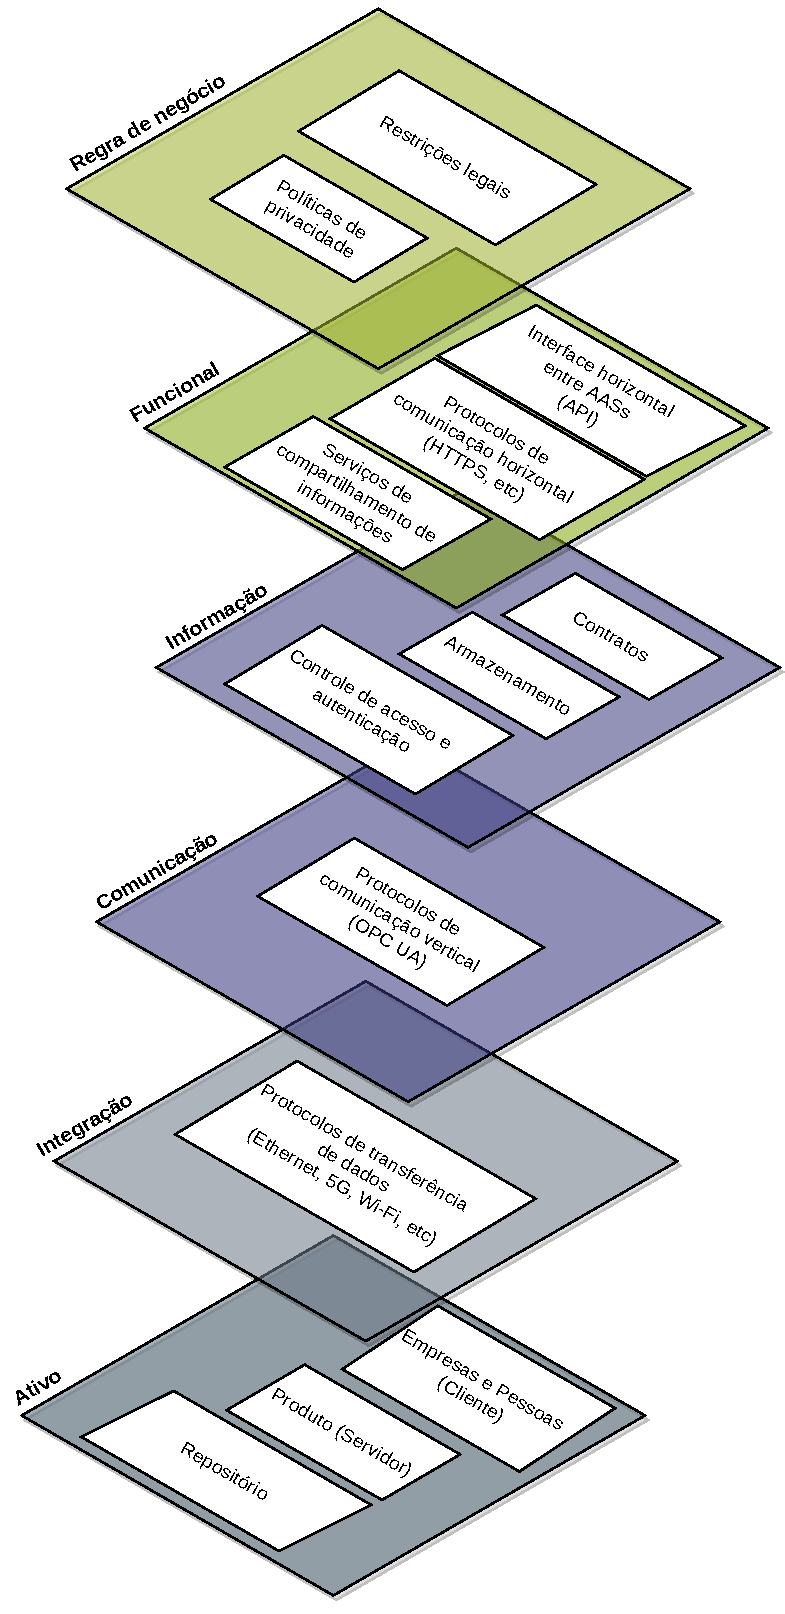
\includegraphics[width=0.8\textwidth]{webservice-rami}
	\caption{Camadas do RAMI4.0 com os elementos da arquitetura proposta.}
	\label{fig:webservice-rami}
\end{figure}

\subsection{Operação de Publicação}

A \autoref{fig:rami-publicacao} apresenta diagramas PFS do fluxo de atividades para a operação de publicação de um C4.0-Servidor em um C4.0-Repositório.

A operação de publicação se inicia sempre que um C4.0 for instalado ou quando esse C4.0 for atualizado.

\begin{figure}[htb]
	\centering
	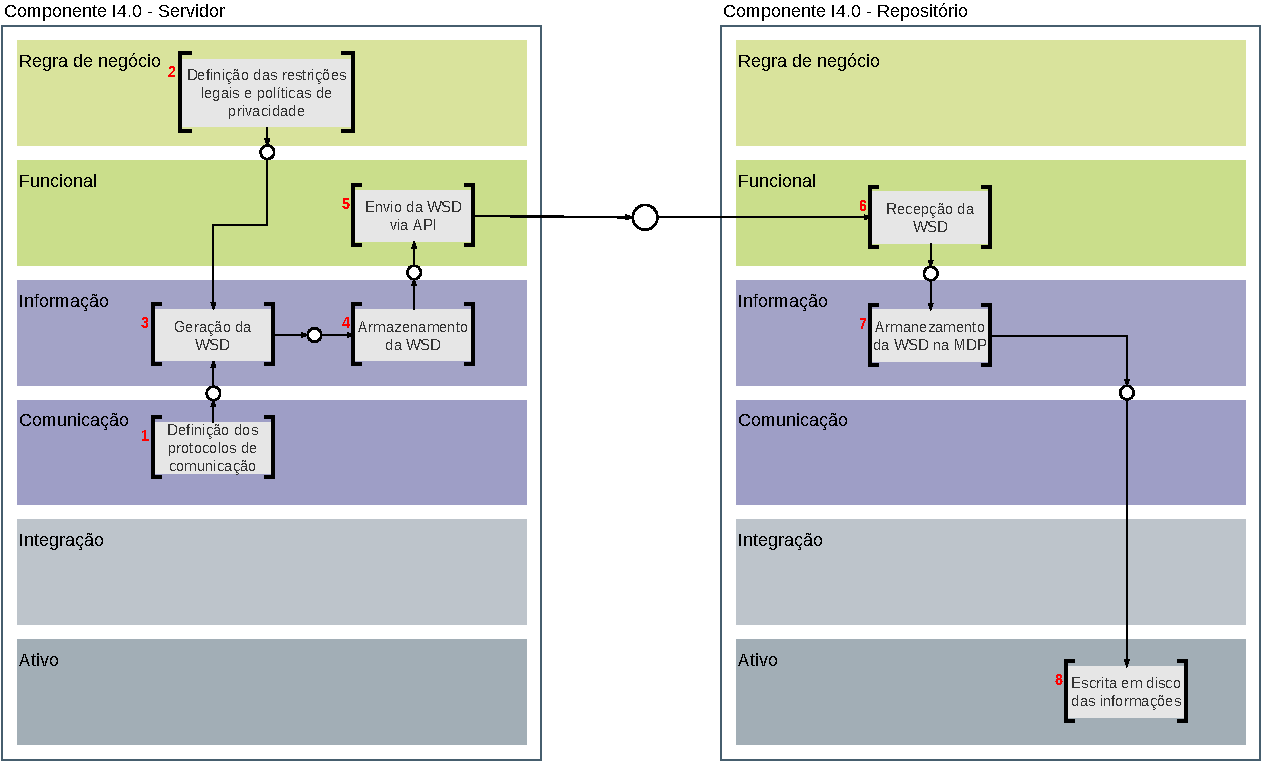
\includegraphics[width=1\textwidth]{rami-publicacao}
	\caption{Diagrama PFS da operação de publicação.}
	\label{fig:rami-publicacao}
\end{figure}

Esta operação é iniciada pelo C4.0-Servidor recém instalado ou atualizado, seguindo um fluxo de atividades estabelecido até chegar no ativo do C4.0-Repositório, os passos são detalhados a seguir:

\begin{enumerate}

	\item Os serviços de compartilhamento de informações do C4.0-Servidor disponíveis são identificados e listados.

	\item As restrições legais e as políticas de privacidade para um determinado C4.0 são acessadas. Esta atividade adicionará restrições aos serviços a serem publicados. Estas restrições serão incorporadas à descrição de cada serviço a ser publicado.

	\item O contrato contendo as descrições de serviços disponíveis no C4.0-Servidor é disponibilizado.

	\item O contrato é enviado ao C4.0-Repositório via API.

	\item O C4.0-Repositório recebe o contrato no formato de intercâmbio definido. A descrição dos serviços nesta fase já contém todas as informações para a identificação do serviço e de seu componente correspondente.

	\item O contrato com a lista das descrições dos serviços é armazenado junto aos demais contratos no \textit{software} ``repositório'' do C4.0-Repositório.

\end{enumerate}

\subsection{Operação de Busca}

A operação de busca é dividida em duas partes: a requisição e a resposta. A requisição é a iniciativa do C4.0-Cliente de requerer a lista de contratos contidas em um C4.0-Repositório, que descreve os serviços de cada ativo cadastrado. O fluxo de atividades da requisição em uma operação de busca é apresentado na \autoref{fig:rami-busca-requisicao}.

Já a resposta da requisição em uma operação de busca é feita pelo C4.0-Repositório para o C4.0-Cliente e é apresentada na \autoref{fig:rami-busca-resposta}.

\begin{figure}[htb]
	\centering
	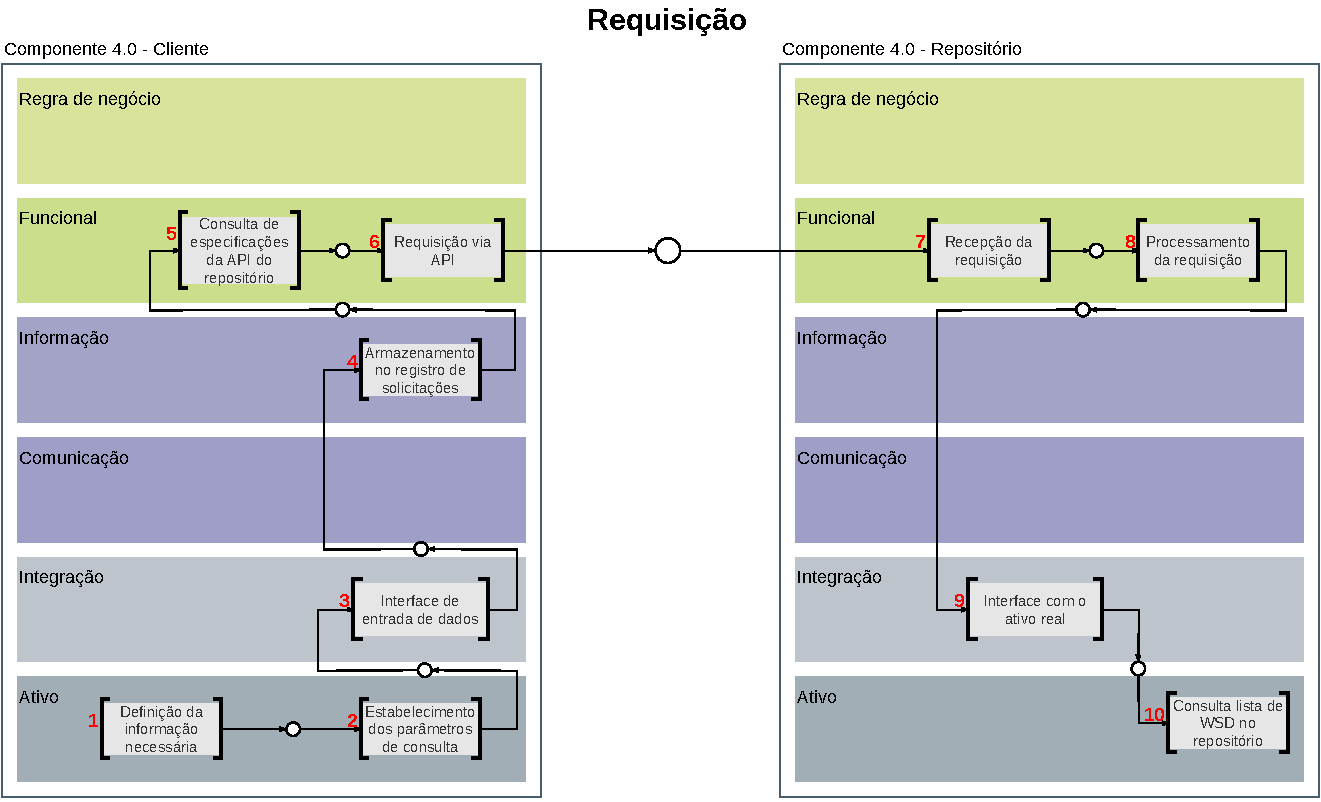
\includegraphics[width=1\textwidth]{rami-busca-requisicao}
	\caption{Diagrama PFS da requisição em uma operação de busca.}
	\label{fig:rami-busca-requisicao}
\end{figure}

A operação de requisição para a busca de um serviço parte do C4.0-Cliente e segue um fluxo estabelecido até chegar ao C4.0-Repositório, esses passos são detalhados a seguir:

\begin{enumerate}

	\item O processo de requisição se inicia com a definição por parte do ativo do C4.0-Cliente (pessoa ou empresa) sobre qual informação se deseja consultar como, por exemplo, leituras de sensores, localização geográfica, manuais, etc.

	\item A partir do tipo de informação a ser consultada, define-se os parâmetros de consulta, que representam o conjunto de restrições que estabelecem qual é exatamente o tipo de serviço que o AAS-Cliente deseja consumir. Para os serviços que visam a extração de informações do ativo, os parâmetros representam, por exemplo, o ID do provedor de serviços, o horário e data de um determinado evento, uma filtragem por modelos específicos de um produto, etc.

	\item Os parâmetros de consulta alimentam uma interface para que a solicitação possa ser virtualizada e integrada ao AAS. Nesta atividade a intenção de solicitação de um serviço é virtualizada.

	\item Opcionalmente, são armazenados os detalhes da solicitação em um registro de solicitações.

	\item A requisição é enviada ao C4.0-Repositório via API.

	\item O C4.0-Repositório recebe a solicitação e a insere ao final da lista de solicitações para ser processada.

	\item A requisição é processada. Identifica-se nesta atividade se a requisição é válida e se ela contém todos os parâmetros necessários para a consulta.

	\item Realiza-se a leitura da lista de contratos no \textit{software} repositório utilizando os parâmetros de consulta estabelecidos.

\end{enumerate}

Após a requisição, o C4.0-Repositório envia a resposta ao C4.0-Cliente. O fluxo de atividades da resposta é apresentada em diagramas PFS na \autoref{fig:rami-busca-resposta}.

\begin{figure}[htb]
	\centering
	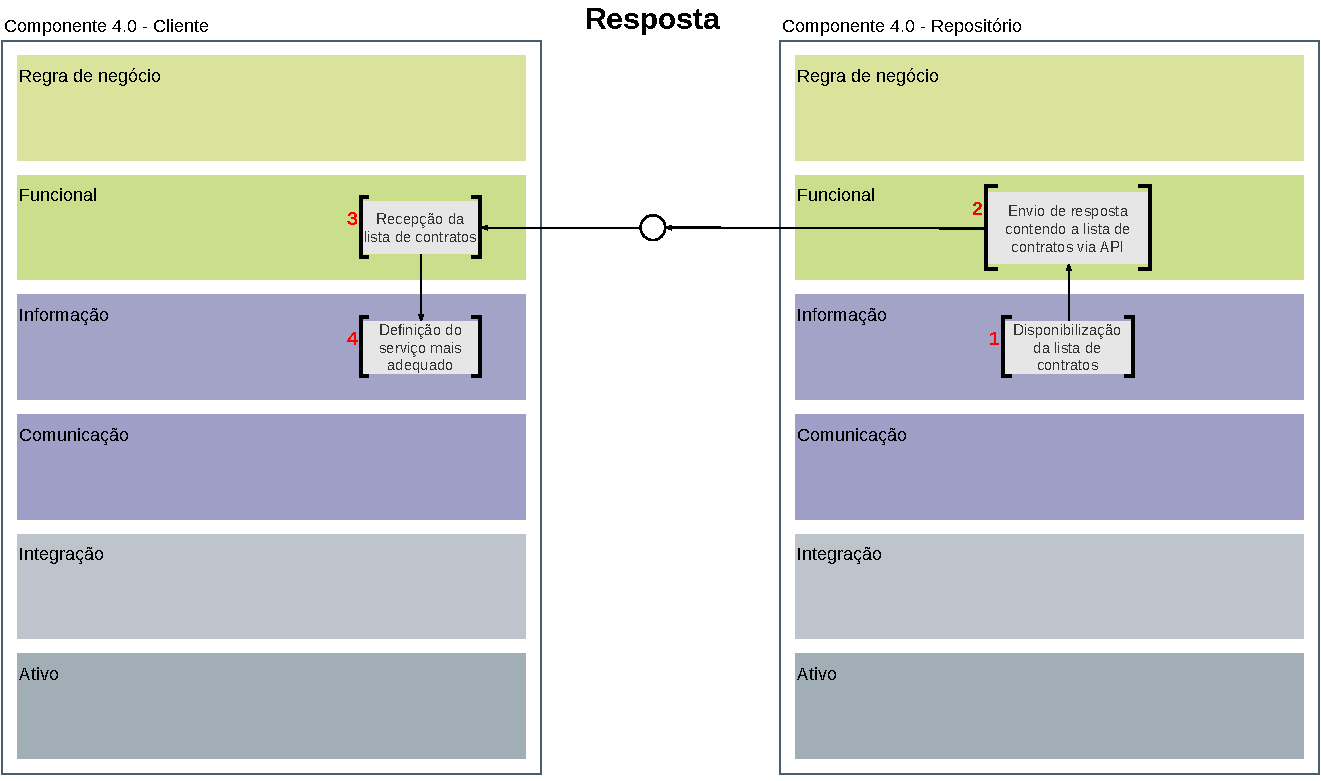
\includegraphics[width=1\textwidth]{rami-busca-resposta}
	\caption{Diagrama PFS da resposta em uma operação de busca.}
	\label{fig:rami-busca-resposta}
\end{figure}

Detalhadamente, a resposta do C4.0-Repositório segue o fluxo de atividades, começando pela disponibilização das informações reais do ativo repositório:

\begin{enumerate}
	\item O contrato contendo a descrições dos serviços é disponibilizado para acesso por parte da camada Funcional. A lista  pode conter serviços válidos, assim como pode conter mensagens de erro por conta de solicitações inválidas ou buscas retornando zero correspondências.

	\item A resposta é enviada ao C4.0-Cliente via API.

	\item O C4.0-Cliente recebe a resposta contendo os contratos no formato de intercâmbio definido.

	\item Após a recepção da lista de contratos contendo todos os serviços disponíveis, é feito o processamento para a definição do serviço mais adequado. Esta fase geralmente não fornece múltiplas opções para a consulta de serviços de compartilhamento de informações ao longo da cadeia de suprimentos uma vez que os parâmetros de consulta na requisição ao repositório geralmente já delimitam exatamente o serviço e o AAS-Servidor que o cliente busca.
\end{enumerate}

\subsection{Operação de Interação}

A operação de interação é a fase final para o consumo de um serviço disponibilizado no mundo conectado da I4.0. Assim como a busca, a interação é divida em requisição e resposta. Primeiramente, o C4.0-Cliente faz uma requisição de consumo de um serviço com parâmetros e então a requisição é processada e respondida pelo C4.0-Servidor.

A \autoref{fig:rami-interacao-requisicao} apresenta o fluxo de atividades em uma requisição de um serviço e a \autoref{fig:rami-interacao-resposta} a resposta do servidor.

\begin{figure}[htb]
	\centering
	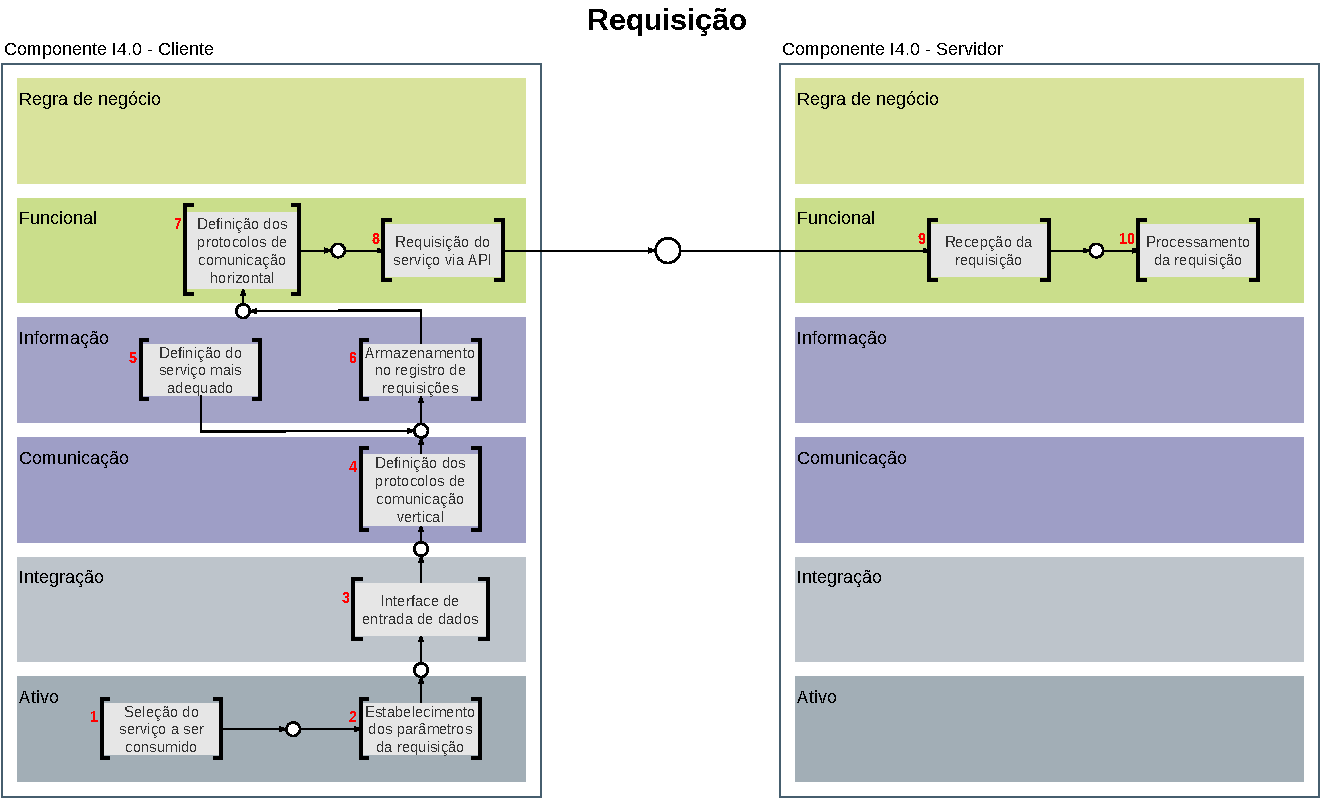
\includegraphics[width=1\textwidth]{rami-interacao-requisicao}
	\caption{Diagrama PFS da requisição de um serviço em uma operação de interação.}
	\label{fig:rami-interacao-requisicao}
\end{figure}

A requisição de um serviço na operação de interação é iniciada pelo C4.0-Cliente e é enviada diretamente ao C4.0-Servidor usando o contrato fornecido pelo C4.0-Repositório. O fluxo de atividades para a requisição de um serviço é detalhada a seguir:

\begin{enumerate}

	\item Surge a necessidade de consumo de uma informação por parte do C4.0-Cliente.

	\item Define-se qual é o serviço mais adequado e de qual C4.0-Servidor será consumido.

	\item As restrições legais e as políticas de privacidade do C4.0-Cliente são consultadas. Essas regras de negócio são incorporadas ao processamento sobre a definição do serviço mais adequado a ser escolhido.

	\item A requisição do serviço é enviada ao C4.0-Servidor via API.

	\item O C4.0-Servidor recebe a requisição e a insere ao final da lista de requisições para ser processada.

	\item É feita a autenticação da identidade do C4.0-Cliente e a autorização para o consumo do serviço. Nesta atividade é verificado se o cliente possui autorização para consumir o serviço e consequentemente os dados que estão sendo solicitados.

	\item Consulta-se as restrições legais e as políticas de privacidade do C4.0-Servidor para a autorização ou bloqueio do fornecimento do serviço ao cliente solicitante.

	\item A requisição é processada. Identifica-se nesta atividade se a requisição é válida e se ela contém todos os parâmetros necessários para o fornecimento do serviço.

\end{enumerate}

Após o recebimento e processamento da requisição de um serviço, o C4.0-Servidor deve fazer a extração e envio das informações de seu próprio ativo. A resposta contendo as informações sobre o ativo começa a partir da emissão de um novo evento ou, caso a informação já esteja disponível na MDP, começa direto da camada de Informação. Esta informação percorre um fluxo padrão para que seja disponibilizada ao C4.0-Cliente por meio do serviço. A \autoref{fig:rami-interacao-resposta} mostra as atividades do fluxo de resposta.

\begin{figure}[htb]
	\centering
	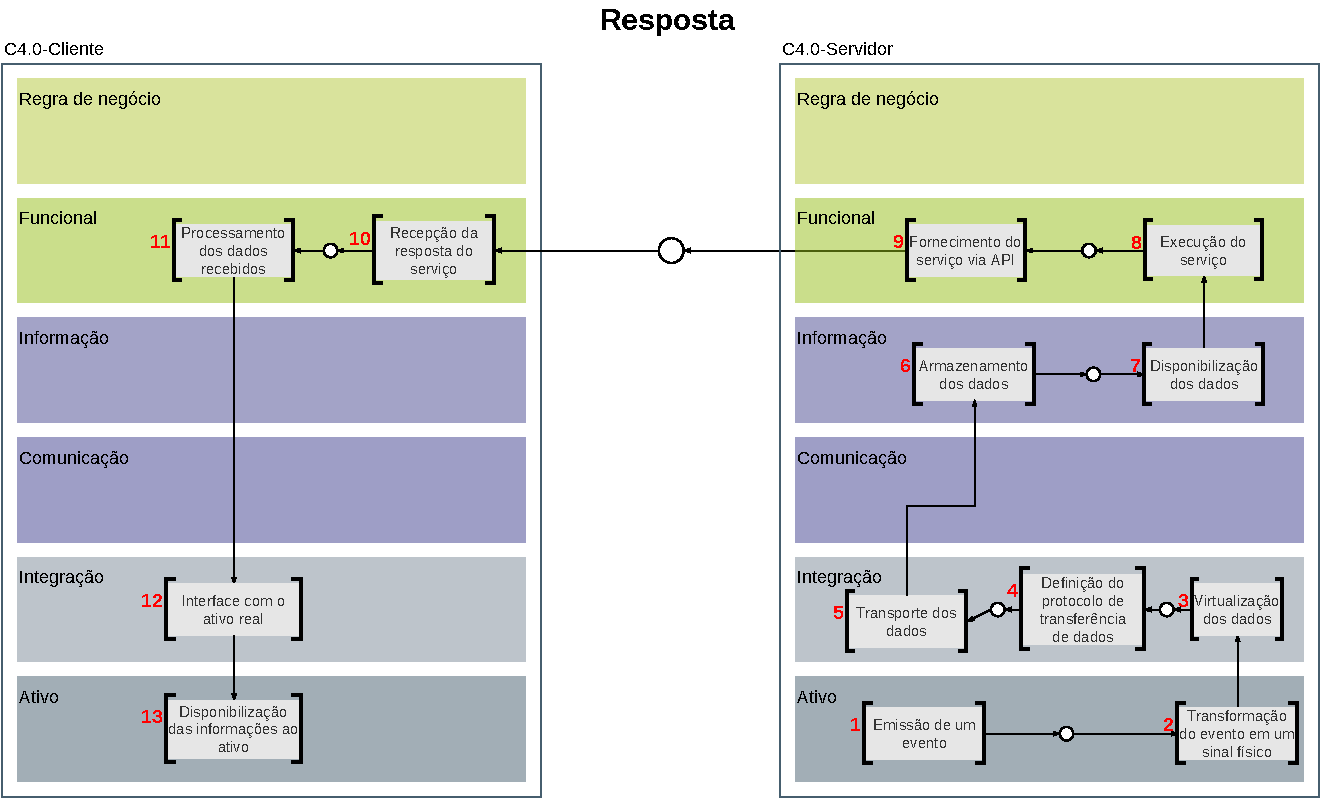
\includegraphics[width=1\textwidth]{rami-interacao-resposta}
	\caption{Diagrama PFS da resposta de um servidor ao se solicitar um serviço.}
	\label{fig:rami-interacao-resposta}
\end{figure}

O detalhamento do fluxo de atividades da resposta é detalhado a seguir:

\begin{enumerate}

	\item Um evento físico no mundo real é emitido.

	\item O evento fornece sinais físicos que podem ser medidos.

	\item Os sinais físicos são interpretados e virtualizados. Nesta atividade é criado um correspondente virtual para o evento do ativo físico, ou seja, os dados são digitalizados e disponibilizados ao AAS.

	\item É definido o meio de transporte e o procolo de transferência de dados como, por exemplo, o Wi-Fi, Ethernet, 5G, etc.

	\item Os dados são devidamente transportados pelo meio e protocolo definidos até uma central de processamento.

	\item Os novos dados sobre o ativo são armazenados pela MDP nos submodelos junto aos demais dados já existentes.

	\item Os dados são disponibilizados ao serviço.

	\item O serviço é executado e sua resposta é gerada. O serviço pode executar quaisquer operações sobre os dados atualizados sobre o ativo assim como sobre o histórico de registros antigos já disponíveis nos submodelos.

	\item A resposta do serviço (fornecimento do serviço) é enviada via API.

	\item O C4.0-Cliente recebe a resposta do serviço em um dos formatos de intercâmbio padronizados \cite{bader2019aas}.

	\item Os dados recebidos na resposta são processados.

	\item As informações geradas alimentam uma interface para comunicação com o ativo real.

	\item As informações do C4.0-Servidor processadas são disponibilizadas ao C4.0-Cliente.
\end{enumerate}

Caso a informação sendo consultada já esteja contida na MDP do C4.0-Servidor (na camada Informação), o fluxo de resposta começa do passo 7, já que neste caso não é necessária a extração dos dados diretamente do ativo (passos 1 -- 6).
